
\documentclass[11 pt,t]{beamer}

\usetheme[
	bullet=circle,		% Other option: square
	bigpagenumber,		% circled page number on lower right
	topline=true,		% colored bar at the top of the frame 
	]{Zurich}


%-----------------------------------------------------------------------------
% DOCUMENT PROPERTIES
\logo{
\includegraphics[scale=0.13]{ouclogo.png}}
\author{DingHao}
\title{Structure of DIP and Fourier Transformation}

%-----------------------------------------------------------------------------


\begin{document}


% ----------------------------------------------------------------------------
\frame{

\titlepage

}
% ----------------------------------------------------------------------------


\section{Example}
\begin{frame}
\frametitle{Contents}
\tableofcontents
\end{frame}

% ----------------------------------------------------------------------------
\begin{frame}
\frametitle{Contents}
\framesubtitle{Handwriting}

\begin{itemize}
    \item Line 1.
    \only<2->{
    \item Line 2.\\
        {\handwriting \textcolor{tangocolordarkchameleon}{Less formal} }
    }
    \only<3->{
    \item Line 3.\\
        {\handwriting \textcolor{tangocolordarkscarletred}{
        Less formal, different color.} }
    }
\end{itemize}


\end{frame}
% ----------------------------------------------------------------------------


% ----------------------------------------------------------------------------
\begin{frame}
\frametitle{Blocks}

\begin{block}{Standard Block}
    This is a standard block.
\end{block}

\begin{exampleblock}{Example Block}
    This is an example block.
\end{exampleblock}

\begin{alertblock}{Alert Block}
    This is an alert block.
\end{alertblock}



\end{frame}
% ----------------------------------------------------------------------------


% ----------------------------------------------------------------------------
\usebackgroundtemplate{
   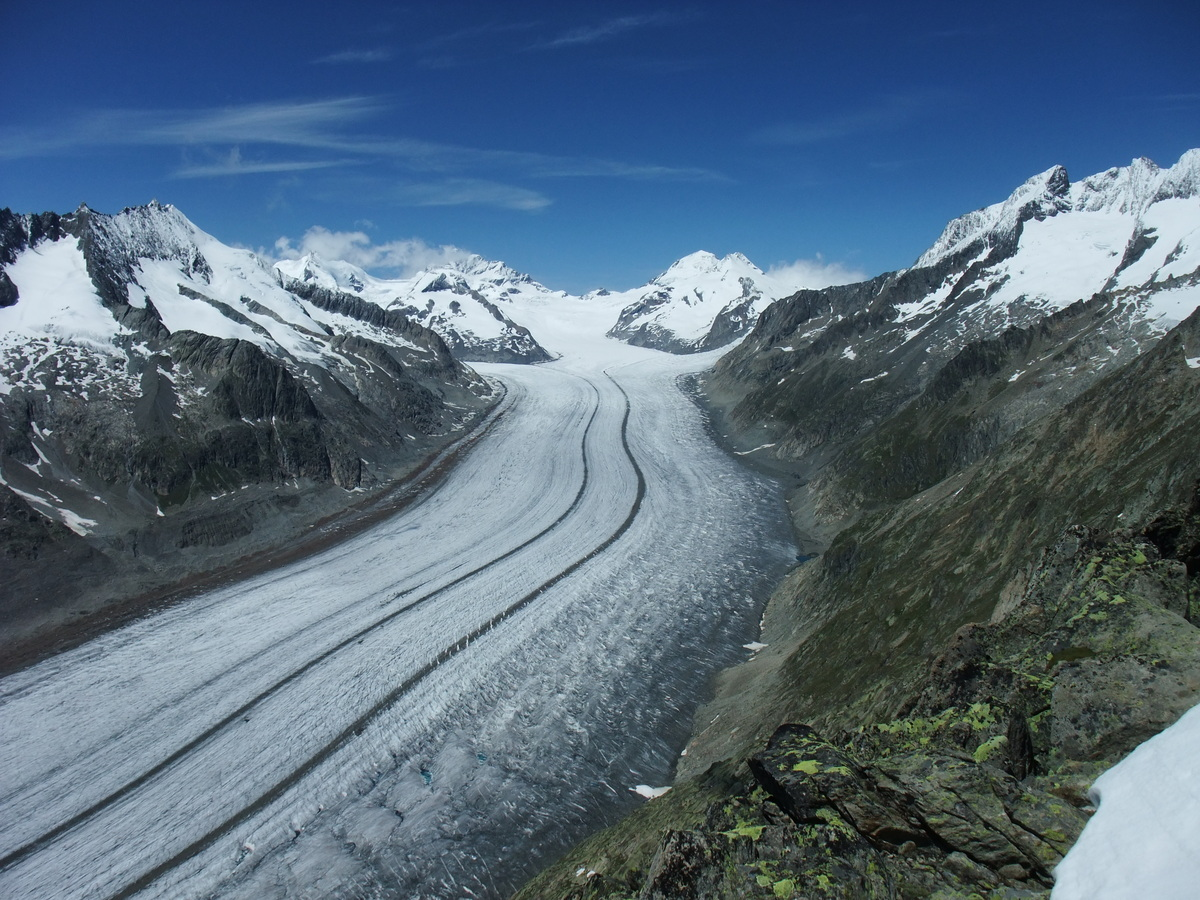
\includegraphics[width=\paperwidth,
                    height=\paperheight]{aletsch}
}
\begin{frame}
\ \\ \ \\
\centering \Large \textcolor{white}{Questions?}

\end{frame}
\usebackgroundtemplate{}
% ----------------------------------------------------------------------------


\end{document}
